\documentclass[12pt]{article}
\usepackage[margin=1in]{geometry}
\usepackage[utf8]{inputenc}
\usepackage{multicol}
\renewcommand{\familydefault}{\sfdefault}
\usepackage{float}
\usepackage{amsmath}
\usepackage{amsfonts}
\usepackage{amssymb}
\usepackage{bm}
\usepackage{graphicx}
\numberwithin{figure}{section}
\usepackage{url}
\usepackage{appendix}

\begin{document}
\begin{center}
\LARGE{Design of an All-Terrain Rover} \\
\normalsize{New Jersey Governor's School of Engineering and Technology}
\end{center}
\begin{multicols}{2}
\noindent \textsc{Tanishq Aggarwal} \\ tanishq.aggarwal.11@gmail.com \\
\\ \textsc{William Li} \\ superwilliamli@yahoo.com \\
\\ \textsc{Abhinav Raghunathan} \\ abhinavr2121@gmail.com
\columnbreak
\\ \textsc{Gargi Sadalgekar} \\ g2sadal@gmail.com \\ 
\\ \textsc{Anita Zirngibl} \\ anita.m.zirngibl@gmail.com 
\end{multicols}
\begin{multicols}{2}
\section*{Abstract}
Ever since the onset of robotics, humans have been finding increasingly clever ways to traverse harsher terrain. Traditionally, two approaches to robotic locomotion have been used: the use of wheels or the use of “legs”. This paper describes the design and construction process of a new type of All-Terrain Rover (ATR) that uses a hybrid design involving both wheels and "legs". The ATR consists of four wheels, with six linear actuators extending radially in a hexagonal pattern from each wheel, as well as two heavy arm-like structures that serve to dynamically alter the center of mass of the vehicle. This design gives the rover significant versatility, allowing it to adapt to both flat terrain (which it can traverse via wheels) and rugged terrain (through the motional flexibility provided by the leg-like actuators.) Using computer-aided design software (CAD), different iterations of the wheel were designed, analyzed using finite element analysis (FEA), and laser cut and put together from wood. A prototype of the wheel has been fully assembled and is ready for testing.
\section{Introduction}
In today’s world, there are two primary methods of robotic locomotion: the use of wheels, and the use of legs, but neither are entirely sufficient in every situation a rover would experience. While wheeled robots are efficient for crossing large, flat landscapes, they struggle when their path contains obstacles that are greater than the radii of their wheels. Legged robots are far more flexible and are capable of crossing a variety of terrain, but also suffer in terms of their physical and software complexity and speed of locomotion.The All-Terrain Rover, or ATR, combines the ideas seen in both wheeled and legged robots in a “hybrid” system. The design of the All-Terrain Rover consists of a four wheel system, with each wheel having the ability to alter its radius via six linear actuators arranged in a symmetric pattern across its diameter. This design is able to handle various obstacles and can help humans in search and rescue missions by driving through the wreckage of natural disasters without risking more lives. It could also be repurposed and used to tackle the uneven geography of Mars. 

This study continues on the heels of many ongoing experimental projects in unconventional robotic locomotion. These projects include BigDog of Boston Dynamics \cite{raibert-bigdog}, and HyQ conducted by Claudio Semini and the University of Genoa \cite{semini-hyq}, both of which focus on optimizing four-legged robots.

The ATR’s wheels include telescopic linear actuators which extend radially from the center of the wheel. The extension and retraction of the actuators act both to move and to stabilize the rover. The rover’s body is also able to dynamically alter its orientation by manipulating its center of mass. The additional functionality provided by the combination of actuators and movable weights afford the rover maneuvering capabilities that far outstrip those of wheeled and legged rovers.
\section{Background}
\subsection{Shortcomings of Wheeled and Legged Robots}
Wheeled robots are far simpler to both build and program than legged ones. Their maneuverability is flexible on a level surface, especially wheels that utilize differential steering and are able to reach high speeds fairly easily.  However, the lack of variety in their locomotive ability hinders the robot in situations that require a higher degree of flexibility (i.e. large obstacles or gaps).

\begin{figure}[H]
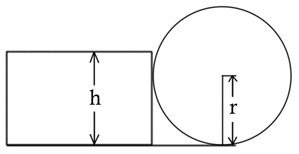
\includegraphics{Height_Limit.PNG}
\caption{The height clearing capabilities are highly dependent on the radius of the wheel. \cite{sanzari-telescopic-actuator}}
\label{fig:height_limit}
\end{figure}

As seen in the diagram above, a wheel is unable to clear a height greater than its radius and will only barely be able to clear one equal to its radius. 

\begin{figure}[H]
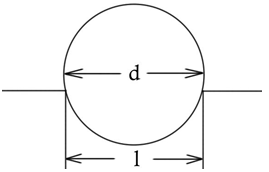
\includegraphics{Gap_Limit.PNG}
\caption{The gap clearing capabilities are highly dependent on the diameter of the wheel. \cite{sanzari-telescopic-actuator}}
\label{fig:gap_limit}
\end{figure}

A wheel is  also unable to cross a gap equal to or larger than its diameter without getting stuck. For these reasons, a wheeled-rover is severely crippled on rough terrain. 

Legged robots have a distinct advantage over wheeled robots in that they are able to climb steps, cross large gaps, and walk on rough terrain by altering their geometry. However, their ability to handle such obstacles comes at the cost of simplicity; legged robots often require complex designs and programming in order to yield the coordination needed for the limbs to function in concert.

In his essay, \textit{Principles of Robotic Motion} \cite{bottcher-locomotion}, Böttcher derives an equation for the total number of lift and release event combinations, $N$, of any legged robot based on the number of its legs, $k$. Lift and release event combinations refer to the combinations of raised and lowered legs where the only two positions possibilities for each leg are raised and lowered. 

\begin{equation}
N = (2k - 1)!
\end{equation}

Based on this equation a four legged robot has 5040 leg positions, only including the lifting and releasing mechanism. Additional joints provide even more flexibility which will require more servos and make programming correspondingly more cumbersome. 

A legged robot, despite having wide degrees of freedom in its leg positions, is still limited in other capacities. For instance, the length which a legged robot is able to travel is always limited by the length of its legs and how fast it can move them, meaning its speed is fundamentally slower than that of a wheeled robot (whose wheels can spin at an almost arbitrary rate). Similarly, a robot can only climb over or onto obstacles shorter than the height of its fully bent leg. These limitations highlight the discrepancy between the high degree of complexity of a legged robot and its limited actual maneuvering capabilities.

A design, therefore, that enables a rover to alter the radius of its wheels by propping it on to extendable leg-like struts, allows the rover to have several types of locomotive function, and thus through this mesh of linear and rotational components, a robot of reasonable simplicity yet significant complexity and speed can be designed.

\subsection{Altering the Rover's Orientation}
In addition to the increased maneuverability provided by the linear actuators, a robot that is able to alter its orientation drastically increases both its height and gap clearing capabilities. A robot that can flip over no longer uses only its wheels to overcome a height and instead uses its entire body. This increases both of the distances (height and gap) that the rover is able to clear immensely. 

\begin{figure}[H]
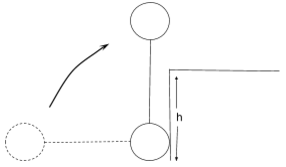
\includegraphics{Flip_Over_Wall.PNG}
\caption{Height clearing capabilities of a rover that is able to alter its orientation.}
\label{fig:flipping-over-wall}
\end{figure}

In order to minimize the torque necessary for the motor to exert when flipping the rover, the center of mass of the rover must be shifted to one wheel axle, which becomes the axis of rotation. The torque necessary to balance to robot on one wheel axle, in preparation for the orientation alteration, is based on equations defining torque:

$$\tau = \bm F \cdot \bm d$$
$$\bm F_r \cdot \bm d_r = F_a \cdot \bm d_a$$

Taking magnitudes, we have
$$M_r g d_r = M_a g d_a$$
\begin{equation}
M_r d_r = M_a d_a
\end{equation}

Where $M_r, M_a$ are the masses of the rover and arm, respectively, and $d_r, d_a$ are the distances from the axis of rotation to the center of mass of the rover and arm, respectively.

\section{Design Process}
\subsection{Wheel Design}
The original concept for the ATR wheel was designed with six telescopic linear actuators that extend from its center. In order for the rover to traverse on actuator legs without the wheel contacting the ground, the actuator has to extend at least twice the length of the radius (Sanzari). The available linear actuators simply could not do this on their own, but the telescopic mechanism doubled the distance of extension of a linear actuator, and coupling the available actuators to the telescopic ones solved the problem (in theory).

\begin{figure}[H]
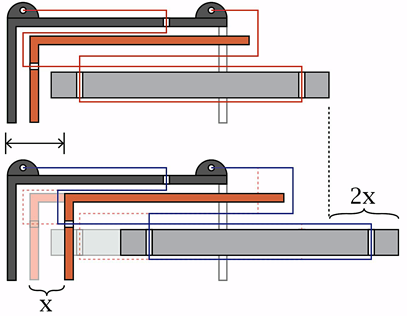
\includegraphics[scale=0.5]{Telescopic_Mechanism.png}
\caption{Telescopic linear actuator design (Sanzari).}
\label{fig:telescopic-actuator-design}
\end{figure}

The telescopic linear actuator is a compound pulley system (see above figure) in reverse. It doubles the extension of the inner actuator via the appendages attached around it. As seen above, the telescopic mechanism requires a string wound around an inner and outer tube, both of which surround the actuator. The string is fed through channels in each of the tubes; these channels act as the surface of pulleys in the compound pulley system.

The problem with this radial design was the sheer amount of material and time needed in order for the wheel to be constructed: each telescopic actuator requires (to describe briefly) an inner tube, an outer tube, plates on either end of the tubes to connect them to each other as well as to the actuator, and string. While the string is not expensive, the process of tying it in a configuration taut enough to allow for the telescopic mechanism to work would be a hugely time-consuming task for 24 separate actuators.

\begin{figure}[H]
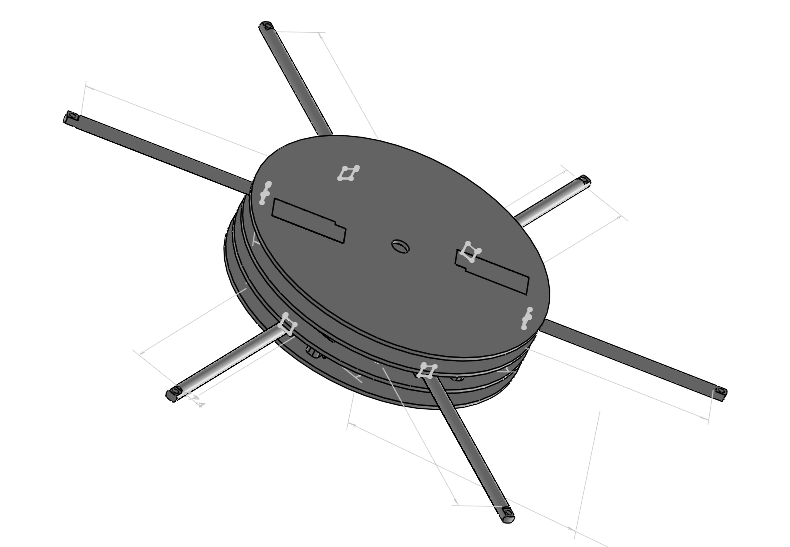
\includegraphics[scale=0.3]{Second_Design.png}
\caption{A CAD of the second wheel design depicting the three layers.}
\label{fig:second_design}
\end{figure}

As a result, the design for the wheel was heavily modified. The second design for the wheel (Figure \ref{fig:second_design} involved layers of circular plates with a pair of (non-telescopic) linear actuators fitted between two layers, yielding a total of three actuator pairs fitted between four circular plates. Within each layer, the two actuators would be placed in opposite directions, with their lengths spanning the diameter of the plate, and each layer’s actuators would form a 60 degree angle with respect to any layer above or below it, so that the overall wheel would have actuators spaced in six symmetrically spaced directions. A foot would be attached to the head of each actuator and fit between the plates. This design was temporarily scrapped (but would later reappear in the final version) due to weaknesses in the foot found via finite element analysis: owing to the width constraints posed on the foot by the small amount of space available between the plates, the design was considered infeasible.

\begin{figure}[H]
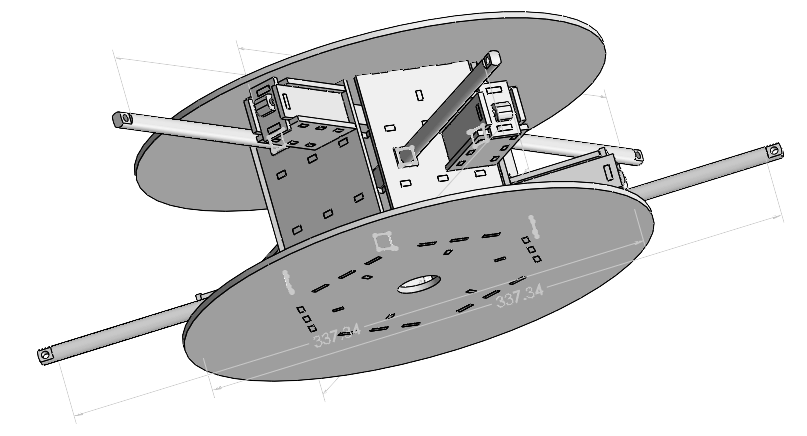
\includegraphics[scale=0.3]{Third_Design.png}
\caption{A CAD of the third wheel design.}
\label{fig:third_design}
\end{figure}

	The third iteration of the wheel consisted of six planks joined in the shape of a hexagon that were sandwiched by two circular plates. Each pair of opposing planks had cutouts that fit around the shafts of a pair of actuators that faced opposite directions and spanned the diameter of the wheel. Attached to the outer face of each plank was a cage that surrounded the actuator body in order to prevent it from falling out. The foot, when attached to the head of the actuator, was intended to fit with the perimeter of the outer plates, so its thickness was no longer significantly limited. However, in order to fit both the foot and the cage within the perimeter of the plates, the diameter of the circular plates needed to be increased. Doing so not only violated materials constraints, but would cause the length that the actuators extended beyond the wheel to decrease to the point that the actuators wouldn’t make contact with the ground.

\begin{figure}[H]
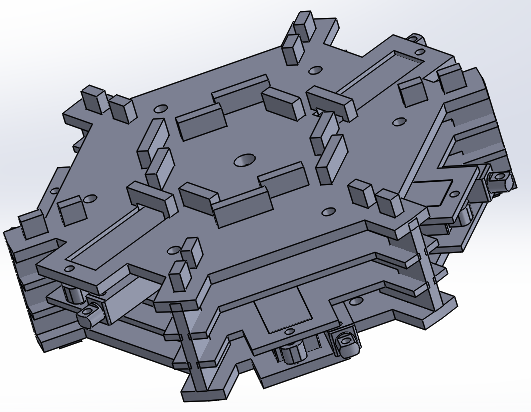
\includegraphics[scale=0.6]{Final_Design.png}
\caption{A CAD of the final wheel design.}
\label{fig:final_wheel_design}
\end{figure}

In the final version (Figure \ref{fig:final_wheel_design}, the base of each actuator is attached to the edge of the wheel, and its body spans the entire diameter of the wheel. In this regard it is similar to the second iteration, except it contains support tabs that enclose the actuator shaft housing and body, as well as E-shaped support elements around the edges of the wheels.

\subsection{Foot Design}
The general design of the foot remained constant throughout the design as an isosceles trapezoid with an arc joined to the larger of the bases. The foot attaches to the actuator head and sits within the perimeter of the wheel when the actuator is retracted. When extended, the actuator pushes the foot outside the wheel perimeter where it makes contact with the ground at about a 30 degree angle. As the design for the wheel changed, the design for the foot had to be adapted. The original design  included a solid foot in the aforementioned configuration that fit between the two face plates. In order to save material and fit into the constraints of newer wheel designs, the solid foot design was replaced with a frame design where two end plates shaped in the original configuration are connected by two side plates that were connected using a tab design. The center and top of the foot are hollow and that part of that space is used to house the actuator head and its connecting pieces (see Figure \ref{fig:final_foot}. 

\begin{figure}[H]
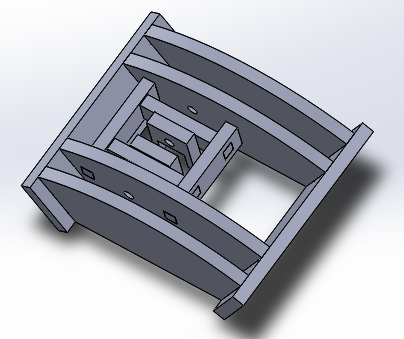
\includegraphics[scale=0.6]{Foot.png}
\caption{A CAD of the final foot design for the central actuators.}
\label{fig:final_foot}
\end{figure}

The assembly in the center of the foot is what the head of the actuator connects to and what provides structure to the rest of the frame.

\subsection{Arm Design}

The original design of the robot included a single arm which provided additional locomotive capabilities. The arm extends from the center of the rover and had 360 degrees of mobility, allowing it to function even when the rover had drastically altered its orientation. The arm design featured double joints, adding another degree of flexibility. The original arm design functions similar to a limb by adding support when needed and using its rigid structure to help the rover overcome large obstacles (see Figure \ref{fig:climbing} for a demonstration of function). 

The revised design for the arm not only alters its design, but is also a major part of its function. In order for the rover to be able to drastically alter its orientation, a certain degree of torque must be applied in order to reduce stress on the arm motor. The arm’s new purpose is to provide this relief. Although a variety of designs were considered, it was decided that the new rover design should include two arms. The arms are both single jointed and are each comprised of a weight that can be moved by a pulley. The arms are attached to the two opposing edges of the chassis (in close proximity to the two wheel axles) and  pass through slits that span the length of the chassis. When the ATR changes its orientation, the arm attached closest to the axis of rotation is rotated so that it extends outside the perimeter of the rover. The weight can then be moved to the end of the arm so that it creates the torque required to flip the rover. This should allow the motor to easily rotate the entire body of the rover about a wheel axle. 

\subsection{Programming}
\subsubsection{Control Flow of Directional/Actuator Commands}
\begin{figure}[H]

\includegraphics[scale=0.15]{Programming_Flowchart.png}
\caption{Diagram representing the flow of information and commands: OpenCV provides wheel position to Python Scripts, which transfers commands to Arduino, which enacts those actions on the actuators and wheels.}
\label{fig:flowchart}
\end{figure}

The ATR is built with a series of programmatic components that interact with each other to allow the operator full control of the rover’s motion. Firstly, the hardware that directly controls the actuators and the wheels is an Arduino board. The board receives commands from a remote computer that issues directions in Python, and transfers these commands to its domain (wheels and actuators). 
\subsubsection{Controlling Actuator Extension Length}
The ATR’s functionality depends heavily on the user’s ability to extend and retract the actuators to specific lengths. To facilitate user experience, the code created accepts a desired extension (in millimeters) and extends to that length. To process the extension amount into an analog output to the actuator, the program uses a function created by Arduino’s map function to transpose the extension length to an analog value.

After multiple trials of testing the extension, a consistent amount of error was observed. The data collected was graphed (see Graph) and a linear line of best fit with an R-squared value of 0.9994 was observed. Using this trend line to transform the input data before mapping, the actuator code yielded accurate extensions with a margin of error around 1 millimeter.

\begin{figure}[H]
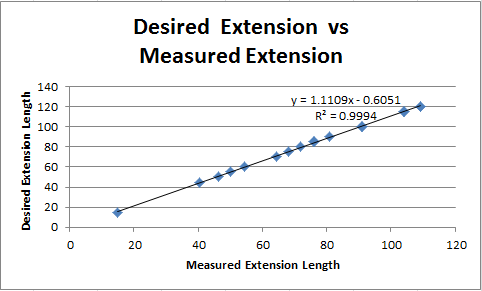
\includegraphics[scale=0.6]{Desired_vs_Measured.PNG}
\caption{Actuator extension calibration results.}
\label{fig:actuator_calibration_graph}
\end{figure}

\subsubsection{Python-Arduino Communication}
Because the Arduino has limited memory and computing power but is useful for processing and relaying low-level commands, a more capable platform was necessary for programming the ATR. Python was chosen for its versatility and its ability to be easily integrated with Arduino and OpenCV. Python was setup to communicate with the Arduino board via Serial, using a code consisting of a sequence of characters and numbers. The user input is processed through a Graphical User Interface written in python, passed to Arduino via the sequence of an alphanumerical sequence, and executed by the actuators.
\subsubsection{OpenCV and Image Processing}
Because the wheel does not have built-in motor encoders, it was necessary to devise an alternate method for determining the exact radial position (in degrees) from the origin. Without any rotational sensors or gyroscopic devices, OpenCV was the best choice for such a task. OpenCV (Open Computer Vision) is a computer vision library that allows a script (written in Python) to get and process individual frames from a live video feed (via webcam positioned behind the wheel) and look for specific symbols to denote positions of the wheel. For example, the origin will have a specific shape that the script can identify and label as the origin.

The mechanism that allows the script to make such a conclusion is called “Contour Matching”. By reducing shapes to their most basic contours and then counting them, a shape can be identified quickly and accurately. Contour Matching is very efficient, and - especially with OpenCV - is easy to implement. By positioning 12 such symbols around the circumference of the wheel, the Python script can detect the rotational position of the wheel and identify which actuators should be extended/retracted at a given time.

\begin{figure}[H]

\includegraphics[scale=0.15]{OpenCV_Part_1.png}
\caption{A sample of three geometric shapes before the “contour reduction” process.}
\label{fig:final_design}
\end{figure}

\begin{figure}[H]

\includegraphics[scale=0.15]{OpenCV_Part_2.png}
\caption{The same sample of geometric figures after “contour reduction” - the line segments (contours) are then counted and used to interpret the shape (colors shown for differentiation)}
\label{fig:final_design}
\end{figure}

In order to maintain the best accuracy and eliminate the chance of any overlap between the symbols on the back of the wheel, it is important to test the size of the field of vision and to orient the camera in a way that allows it to focus on only one symbol and not its neighboring symbols. In this way, the camera was calibrated to detect only one image that is easily readable.
\subsubsection{Graphical User Interface}
In addition to the script that actually controls the actuators/wheels, software to easily edit the speed of the wheel and the retraction/extension distance for the actuators is crucial. Continuing the use of Python within the software side, a Graphical User Interface (GUI) was developed. The GUI, written in Python, provides an easy way to select an actuator and extend/retract it with a specified distance. The actuator is located by Wheel Number (\#1 through \#4) and Actuator Letter (A - F). Furthermore, the GUI contains the trigger for the Python-Arduino interaction (explained in “Python and Arduino Communication”). In addition, the GUI graphically shows the radial position of the wheels with regard to the origin with a degree measure from the OpenCV Python script (explained “OpenCV and Image Processing”). With this information, it becomes possible to correctly select the actuator that needs to be extended/retracted for the robot to continue its motion.

\subsection{Electrical Integration}
One of the obstacles with building the ATR is the problem of connecting wires from a stationary frame to rotating wheels. A direct, wired connection would result in the twisting of wires, so slip rings are needed for attachment. Slip rings have an inner cylinder and an outer shell that rotate around each other. By keeping the inner cylinder fixed to the wheel axle and allowing the outer shell rotate with the wheel, the wheel can spin (relative to the ATR) without having its wires becoming entangled. 

\section{Assembly Process}
The majority of the wheel structure is laser cut from baltic birch wood. The assembly of the laser cut wood parts is completed in specific order so that all the parts to assume their proper positions within the structure. First, the inner support structures and inner base structures are inserted into the inner two plates. Then the actuators are inserted before the ‘E’ support structures are added to the edges of the plates. Finally, the outer plates enclose either side of the wheel.  Some problems with constructions are the flaws  When fully assembled, the tight fit of the parts create enough friction to hold the wheel together without any bolts. However, bolts are inserted through the wheel for additional security. The body of the robot was constructed using VEX Robotics parts. Stepper motors were used to power the wheels and arms. 

\section{Results}
\subsection{Currently available results}
The rover wheel was sufficiently stable even without additional bolts (i.e. it held together due to the friction between puzzle pieces). It was also slightly heavier than expected. 
\subsection{Further Testing}
\subsubsection{Height Clearing Capabilities}
The rover’s height clearing capabilities will be tested by having the rover drive over heights starting at 110 mm, the radius of the wheel, and increasing in increments of 10 mm in order to gauge the maximum height that the rover can clear. A height would be declared successfully cleared when the rover was able to cross it with a success rate of 90\% .
\subsubsection{Gap Clearing Capabilities}
The rover’s gap clearing capabilities will be tested by programming the rover to cross a gaps of various widths. The widths will begin at 220 mm, the diameter of the wheel without extended linear actuators. The widths will be increased at increments of 20 mm until the rover is no longer able to successfully clear the gap. A gap will be declared successfully cleared when the rover is able to clear it with an 90\% success rate. 
\subsubsection{Various Terrains}
The rover is designed to be able to navigate a variety of terrains.  The success of the rover on each terrain will be measured by the distance that the rover travels in 60 seconds. These terrains will include a flat surface (i.e. a floor), a rough surface (i.e. a bed of gravel), and a soft surface (i.e. mud).

\section{Conclusion}
The design for a wheel with linear actuators can be constructed using a press fit. The design of the wheel is effective because it resulted in a wheel that is structurally sound on all sides, while allowing the actuators to extend to the necessary length past the wheel.
\subsection{Further Steps}
The puzzle-like design of the wheels was adopted in order to simplify construction and reduce the number of bolts and screws. While the wheels produced from this concept were fairly sturdy, they are likely not rugged enough for use in field operations. Later iterations of the wheel need to be redesigned with tougher materials and better attachment methods. In addition, the chassis of the ATR is constructed from VEX robotics parts, but a future version should be constructed from specially designed parts to maximize material efficiency.

From a software point of view, automation is a major step forward in the future. Even if the robot does not become fully autonomous, patterns of code should be developed for predictable scenarios, such as crossing a gap or climbing a cliff. To increase the ATR’s capabilities, more sensors need to be connected. For example, distance sensors will help the ATR detect obstacles in its path and predict the correct maneuver to perform. With more sensors, the robot can observe its environment and learn to match maneuvers to scenarios.

\section{Acknowledgments}
The authors gratefully acknowledge Michael Sanzari of Rutgers University, whose technical experience and knowledge of engineering proved to be extremely essential to this study. The authors also thank the Rutgers University branch of the IEEE for allowing them to use their facilities and resources. The authors appreciate the work of the Makerspace workers who helped laser cut the wheel parts. 

The authors would like to take this time to thank Rutgers University’s Wireless Information Network Lab (WINLAB), which generously allowed the authors to use their equipment and facilities. The authors sincerely appreciate the efforts of Charles McGrew from Hackerspace, who loaned the linear actuators that made this entire concept possible. The authors would also like to thank Alexander Hobbs, who aided research as project mentor by providing transportation and guidance, and to the New Jersey Governor’s School of Engineering and Technology, the program under which this research was conducted. Finally, the authors would like to thank the dean of the program, Ilene Rosen, and Assistant Dean Jean Antoine Patrick for their support and review of the project through the program, as well as sponsors of the GSET program for making the program possible.
\section{References}
\begin{thebibliography}{4}
\bibitem{raibert-bigdog} 
M. Raibert, K. Blankespoor, G. Nelson, et. al, “BigDog, the Rough-Terrain Quaduped Robot” , Boston Dynamics, Waltham, MA, 2008.
 
\bibitem{semini-hyq} 
C. Semini, “HyQ - Design and Development of a Hydraulically Actuated Quadruped” , Ph.D. dissertation, Dept. Advanced Robotics, Univ. Genoa, Italy, 2010.
 
\bibitem{sanzari-telescopic-actuator} 
M. Sanzari, “Experimental Mars Rover Design: Telescopic Linear Actuators”, term paper, Rutgers’ School of Engineering, 2016, (unpublished)

\bibitem{bottcher-locomotion} 
S. Böttcher, “Principles of robotic locomotion”, 6-7, WWW Document (\url{http://www2.cs.siu.edu/~hexmoor/classes/CS404-S09/RobotLocomotion.pdf})
\end{thebibliography}
\end{multicols}

\begin{appendices}
\section{Figures}
\begin{figure}[H]
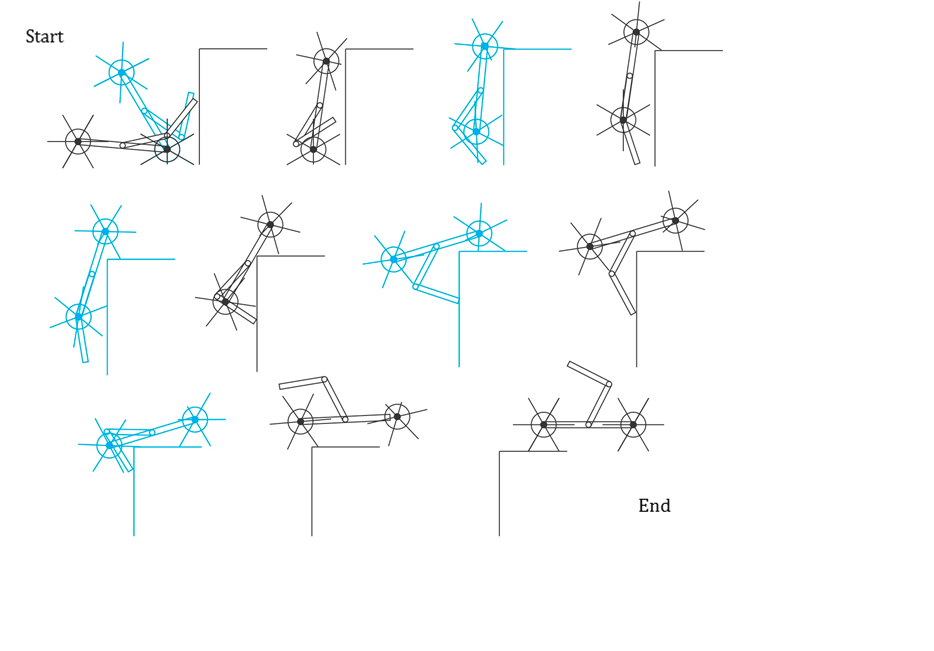
\includegraphics[scale=0.6]{Climbing_Diagram.png}
\caption{A diagram depicting a potential use for the arm \cite{sanzari-telescopic-actuator}}
\label{fig:climbing}
\end{figure}
\end{appendices}

\end{document}